%%=============================================================================
%% Methodologie
%%=============================================================================
\graphicspath{{graphics/}}
\chapter{\IfLanguageName{dutch}{Methodologie}{Methodology}}%
\label{ch:methodologie}

\section{Stap 1: Bestaande oplossingen vinden}
In de eerste fase van het onderzoek zal er een literatuurstudie worden gedaan over het maken van een driver, MiFare- en smartcards en de card reader. Dit zal de eerste vier weken gebeuren. Het is de bedoeling dat er hieruit al één of meerdere manieren worden gevonden die mogelijks de onderzoeksvraag kunnen beantwoorden later in het onderzoek.

\section{Stap 2: Interview met Anton D'hondt}
Er is geen zekerheid dat er manieren worden gevonden in stap 1. Daarom zal er ook een interview worden afgelegd met Anton D'hondt. Hij heeft het idee voor een mogelijke oplossing met behulp van Windows Services en SignalR.

\section{Stap 3: Oplossingen uitwerken}
Vervolgens zal er een vergelijkende studie worden gedaan om te kijken welke mogelijke oplossing het beste is. Zowel WebUSB als het idee van de Anton D'hondt zullen hiervoor (indien mogelijk) worden uitgewerkt tot een Proof of Concept. Deze Proof of Concept zal Jan De Nul dan kunnen gebruiken om smartcards in te lezen op hun webapplicatie.

\section{Stap 4: Succes bepalen}
Bij het bepalen van succes voor deze Proof of Concepts zal worden rekening gehouden met twee factoren. Enerzijds zal de Proof of Concept moeten werken en anderzijds zal de tag in minder dan een seconde moeten kunnen verschijnen in de webapplicatie. Er zal geen rekening worden gehouden met de veiligheid omdat de Proof of Concept enkel binnen het Jan De Nul netwerk zal worden gebruikt en dus niets zal versturen over het internet.


\graphicspath{{graphics/}}
\chapter{\IfLanguageName{dutch}{Onderzoek en Proof of Concept}{Research and Proof of Concept}}%
\label{ch:Onderzoek en Proof of Concept}
\section{Inleiding}
Wat is nu de beste manier om een card reader te verbinden met een webapplicatie? In dit hoofdstuk zal er stap voor stap worden uitgelegd hoe er op deze vraag een oplossing is gevonden. Er zal gesproken worden over WebUSB en SignalR, waarom er voor een van die twee gekozen is als oplossing tot de onderzoeksvraag en hoe deze oplossing uitgewerkt wordt in een Proof of Concept voor Jan De Nul.

In dit hoofdstuk zullen dus de stappen van de methodologie worden uitgevoerd. Om het duidelijk te houden is het opgesplitst in twee delen, een deel over WebUSB en een deel over SignalR. Voor het deel over SignalR gaat het interview met Anton D'hondt nog worden besproken. In beide delen zal worden gekeken of deze mogelijke oplossingen voldoen aan de vooropgestelde factoren. 
Eerst zal er in volgende tussentitel de mogelijke oplossingen eens worden besproken.


\section{De twee mogelijke oplossingen}
Eerst is er op het internet op zoek gegaan naar welke mogelijke oplossingen er zijn om een card reader rechtstreeks te verbinden met een website. Hierbij werd al snel duidelijk dat WebUSB de enige oplossing is waarbij de card reader ook echt rechtstreeks met de browser verbonden zou zijn. In het volgende hoofdstuk van dit onderzoek gaat deze manier dan ook worden uitgetest. Echter bleek uit die test en nog wat verder onderzoek dat deze manier niet werkt voor card readers. Waarom dit is zal meer gedetailleerd uitgelegd worden in het volgende hoofdstuk. 

Er is dus nog gezocht naar een andere oplossing. Deze oplossing is bekend geraakt door een interview met Anton D’hondt. Hij had het idee om gebruik te maken van SignalR en Windows Services. Het idee is geïnspireerd op eID software, dat wordt gebruikt door ItsMe. Maar in plaats van het gebruik van een extensie, zoals eID software doet, wordt er hier gebruik gemaakt van SignalR om de data maar de website te versturen. Ook hier gaat in detail over gesproken worden in verdere hoofdstukken. 



\section{WebUSB als oplossing}

\subsection{Inleiding}
WebUSB is de eerste mogelijke oplossing die opkwam om deze onderzoeksvraag te beantwoorden. Zoals eerder al vermeld in de literatuurstudie is WebUSB zeer handig om USB-apparaten te verbinden met, en rechten te geven aan een website. Het plan was dus om te testen of WebUSB een oplossing is voor het gebruik van een card reader op een website.

\subsection{Test project met WebUSB}
Om dit te testen is er een klein projectje opgesteld waarin WebUSB wordt gedemonstreerd. Dit projectje bestaat uit een simpele HTML file en een typescript file.  De HTML file zal een simpele titel en een knop bevatten. Wanneer er op die knop gedrukt wordt zal de ´connectDevice()´ command aangeroepen worden. 

HTML: 
\begin{verbatim} 
    
    <h1>Press the button to test device connection</h1> 
    <button (click)="connectDevice()">Connect a device</button> 
    
\end{verbatim} 

De ´connectDevice()´ command werkt als volgt. Er zal als eerste gebruik worden gemaakt van ‘navigator[‘usb’]’, dit is een property van het 'navigator’ object in het environment van de webbrowser. Als de WebUSB API wordt ondersteund door de browser zal ‘navigator[‘usb’]’ een object teruggeven dat kan worden gebruikt om toegang te krijgen tot USB devices. Als de WebUSB API niet ondersteund wordt door de browser dan zal dit een undefined error teruggeven bij het aanroepen van ‘navigator[‘usb’]’. Browsers zoals Chrome, Firefox, Microsoft Edge en Opera ondersteunen WebUSB, maar Safari niet. 

Via ‘navigator[‘usb’]’ kan er dan vervolgens de ‘connectDevice()’ functie worden aangeroepen. Deze functie gaat ervoor zorgen dat er een pop-up schermpje tevoorschijn komt met daarin alle USB-apparaten die verbonden zijn met de computer. Handig om te weten is dat er ook filters kunnen aan worden meegegeven, zoals vendorId of productId. Deze filters moeten worden meegegeven binnen de ´{ }´. In het geval van dit projectje wordt er geen gebruik gemaakt van deze filters omdat het nog onnodig is voor dit test projectje, dit wordt gedaan door de { } leeg te laten. De ‘requestDevice’ functie geeft het geselecteerde apparaat terug. Met behulp van de ‘.then’ functie, waarin het ‘selectedDevice’ het geselecteerde apparaat voorstelt, kunnen er vervolgens verdere verwerkingen worden uitgevoerd met het ‘selectedDevice’. In dit projectje gaat er om de verbinding te testen gebruik worden gemaakt van een simpele ‘console.log(selectedDevice)’ om indien de verbinding er is de apparaat data te loggen in de console. 

Typescript: 
\begin{verbatim} 
    
    async connectDevice(): Promise<any> { 
        
        navigator['usb'] 
        
        .requestDevice({ filters: [{}] }) 
        
        .then((selectedDevice) => { 
            
            console.log(selectedDevice); 
            
        }) 
        
        .catch((error) => { 
            
            console.log(error); 
            
            alert(error); 
            
        }); 
        
    } 
    
\end{verbatim} 

\subsection{Waarom geen WebUSB}
Als de bovenliggende code wordt uitgevoerd zal er dus een pop-up verschijnen met daarin alle USB-apparaten die met de computer verbonden zijn.

\begin{center}
    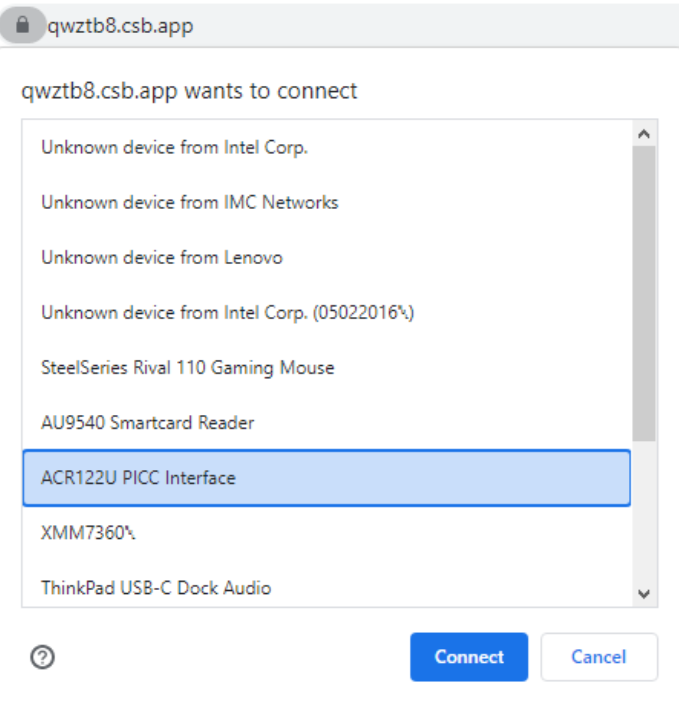
\includegraphics[width=8cm]{device_list}
\end{center}

Als er in de lijst dan de ACR122U cardreader wordt geselecteerd, dan zal de informatie over deze card reader in de console worden gelogd. Dit werkt allemaal zoals het hoort te werken.

\begin{center}
    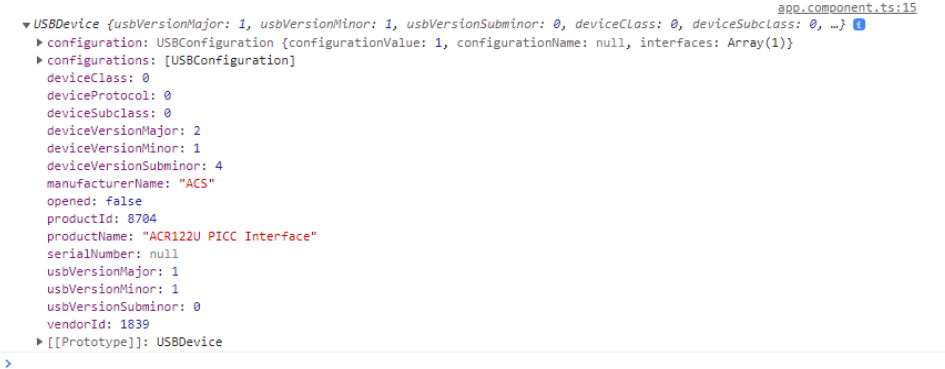
\includegraphics[width=16cm]{device_log}
\end{center}

Maar om ook echt de connectie te maken met de card reader, zodat de kaart kan worden uitgelezen, moet het geselecteerde device geopend worden. Dit kan ongeveer op dezelfde manier als in de code hierboven. Maar in plaats van het device te loggen in de console zal de ‘open()’ functie hierop worden uitgevoerd. Deze zou een promise terug moeten geven die duidelijk maakt wanneer de sessie op het USB-apparaat is gestart. Dit geeft volgende error terug: 

\begin{center}
    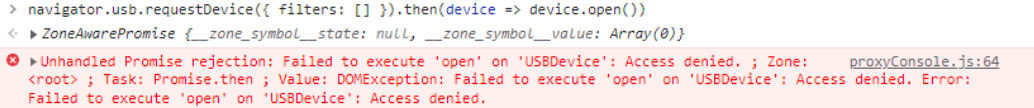
\includegraphics[width=16cm]{webusb_error}
\end{center}

Na verder onderzoek over deze error blijkt dat deze error wordt gegooid om veiligheidsredenen. Volgens \textcite{ReillyGrant} zijn er buiten de Smart Card interface class nog enkele andere interface classes die worden geblokkeerd bij het gebruik van WebUSB. Dit zijn de Audio, Video, HID, Mass Storage en tenslotte ook nog Wireless Controller (Bluetooth en Wireless USB) classes. Deze interface classes worden in de eerste plaats al vaak geblokkeerd door de ingebouwde class drivers van besturingssystemen. Door deze dus ook te blokkeren voor WebUSB zorgt dit voor consistentie over de verschillende platforms. 

Waarom vormen deze device classes dan een risico voor de veiligheid van gegevens? Sommige device classes kunnen een beveiligingsprobleem vormen voor WebUSB omdat ze niet bedoeld zijn voor algemeen gebruik en kunnen gevoelige informatie bevatten. Wanneer een apparaat via WebUSB toegankelijk wordt gemaakt, kan de inhoud ervan worden gelezen of gewijzigd worden door de webapplicatie die toegang heeft gekregen. 

Als het apparaat, dat zoals in dit geval een smartcard reader is, zou het lezen of wijzigen van de inhoud door een webapplicatie met kwaadaardige bedoelingen tot identiteitsdiefstal kunnen leiden. In dit geval is het belangrijk om ervoor te zorgen dat alleen bevoegde partijen toegang hebben tot de smartcard reader en dat de communicatie tussen de webapplicatie en het apparaat veilig is. Als een apparaat een device class heeft die als beveiligingsrisico wordt beschouwd, is het aan de fabrikant van het apparaat om het apparaat te beveiligen tegen onbevoegde toegang.

Deze manier voldoet niet aan de factor dat het moet werken en is dus geen oplossing tot de onderzoeksvraag.




\section{Interview voor tweede oplossing}
Terwijl er werd uitgetest of WebUSB een goede oplossing zou zijn werd er al op zoek gegaan naar een tweede oplossing. Voor deze tweede oplossing was het plan om een interview te doen met iemand die verstand heeft van hoe de kaart lezer via een omweggetje (omdat WebUSB geen oplossing bleek te zijn) kan verbonden en uitgelezen worden met een webapplicatie. Hiervoor bleek Anton D’hondt de geschikte persoon te zijn. Anton werkt bij Jan De Nul en is er lead developer in het HR-team. 

Er werd Anton gevraagd hoe hij dit probleem zou aanpakken en hij kwam met een idee dat gebaseerd is op hoe eID tewerk gaat. 

Belgium eID software is een set van softwareprogramma's die nodig zijn om de Belgische elektronische identiteitskaart (eID) te gebruiken. Het is ontwikkeld door de Belgische overheid om het gebruik van de eID te vereenvoudigen. 

Hoe eID exact werkt is niet geweten. Anton speculeert dat eID gebruik maakt van hun eigen applicatie en een extensie. Deze applicatie en extensie staan dan eigenlijk in verbinding met elkaar. De applicatie stuurt de data van de kaart door naar de extensie en deze extensie gaat er vervolgens voor zorgen dat de data op de website terecht komt. Hierbij moet wel onthouden worden dat het slechts speculaties zijn, aan de hand van wat ze de gebruiker doen downloaden (hun applicatie) en de extensie die de gebruiker moet installeren in de browser. 

Het idee van Anton zal als volgt werken. In de eerste plaats zal de kaart moeten kunnen uitgelezen worden telkens dat er een kaart tegen de card reader wordt gehouden. Hiervoor gaat er dus gebruik worden gemaakt van een Windows Service. Deze keuze is omdat een Windows Service over lange tijd kan werken en het de gebruiker niet stoort als die met andere dingen bezig is (omdat het op de achtergrond, zonder user interface werkt). De code voor het inlezen van de MiFare kaart zal dus in de Windows Service worden geplaatst. In de tweede stap zal gebruik worden gemaakt van SignalR. Deze gaat met behulp van Server-sent Events de data van de Windows Service naar de website transporteren. Het gaat dus eigenlijk dienen als een soort tussenstuk. En als laatste stap zal de data van de kaart worden opgevangen in de webapplicatie. En dus telkens dat er een nieuwe kaart wordt gescand, zal deze zichtbaar worden op de webapplicatie. 

Waarom wordt er dan geen gebruik gemaakt van een extensie zoals eID het doet? Dit is omdat er geen echt framework bestaat om cross platform extensions te schrijven. Bovendien is dit ook nog een ander environment dat moet aangeleerd worden wat de codebase complexer maakt.




\section{SignalR en Windows Services als oplossing}

\subsection{Inleiding}
Nu zal er dus stap voor stap getoond worden hoe het idee van Anton uitgewerkt wordt. Er zal begonnen worden met het uitlezen van de kaart in een Windows Service. Vervolgens zal er getoond worden hoe de SignalR Hub werkt. En tenslotte zal de verbinding tussen de SignalR hub en webapplicatie volgen.   

In de Windows Service zullen er soms methodes voorbij komen die te maken hebben met het uitlezen van de kaart. Aangezien dit buiten de scope van deze bachelorproef valt zal hier geen gedetailleerde code over getoond worden. 

Hieronder is er een schema dat een beetje meer duidelijkheid moet brengen over hoe het idee in elkaar zit. 

\begin{center}
    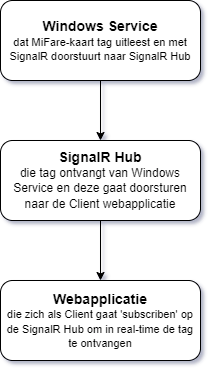
\includegraphics[width=6cm]{BP_voorbeeld_schema}
\end{center}

\subsection{Kaart uitlezen met Windows Service}
De eerste stap om het idee van Anton uit te werken is het maken van een Windows Service.  

Dit wordt gedaan door een class te maken, bijvoorbeeld 'Worker’, en deze de ‘IHostedService’ interface te laten implementeren. Deze interface gaat twee methods definiëren, de 'StartAsync’ en de ‘StopAsync’ methods. De StartAsync gaat worden uitgevoerd wanneer de service wordt gestart en de StopAsync wanneer de service wordt afgesloten.  

De Worker heeft een ‘ILogger’ als property, en deze wordt gedeclareerd in de constructor. Met behulp van de ILogger kunnen ontwikkelaars belangrijke informatie over de status en prestaties van hun achtergrondtaken of services vastleggen en analyseren. Zo kunnen logs bijvoorbeeld worden gebruikt om te controleren of de service wel goed is opgestart en of er fouten zijn opgetreden tijdens het uitvoeren van de service. Een tweede property is de ‘monitor’, dit is een instantie van de SCardMonitor class.  SCardMonitor is een class die wordt gebruikt om smartcardgebeurtenissen te monitoren en af te handelen. Het biedt de mogelijkheid om smartcardgebeurtenissen in realtime te volgen en te reageren op deze gebeurtenissen, zoals kaartinvoer en -verwijdering.

Dan wordt de 'StartAsync’ methode geïmplementeerd. Deze methode zal worden opgeroepen op het moment dat de service wordt opgestart. Binnen die methode zal er eerst de naam van de card reader worden opgehaald. Dit gebeurt aan de hand van de 'GetCardReader’ methode. Deze methode gaat bekijken welke card readers er allemaal verbonden zijn met de computer om vervolgens de juiste card reader uit de lijst te halen en deze terug te geven. Hiervan gaat de code echter niet worden besproken aangezien dit dus buiten de scope van de bachelorproef valt. Nadat de card reader is teruggegeven zal er met behulp van de monitor (een instantie van SCardMonitor) voor worden gezorgd dat er telkens dat er een kaart tegen de card reader wordt gehouden hiervan de tag wordt uitgelezen. Er wordt met 'monitor.CardInserted’ dus eigenlijk gezegd dat telkens een kaart wordt gelezen, de methode die wordt meegegeven moet worden uitgevoerd. In dit geval de 'GetUID’ method die de tag van de kaart gaat uitlezen, gaat omvormen naar een string en deze dan gaat versturen met behulp van SignalR. Hierover komt verderop nog meer uitleg. Tenslotte wordt de monitor gestart en zal door de card reader naam mee te geven de juiste card reader worden uitgelezen. Dit gebeurt met de ‘monitor.Start(readerName)’ method. 

Nu zal vanaf de 'StartAsync’ wordt aangeroepen een connectie bestaan met de card reader. 

Om de Windows Service te stoppen bestaat er ook de ‘StopAsync’. Deze method zal zoals eerder gezegd worden uitgevoerd wanneer een service wordt afgesloten. Binnen deze method gaan de ‘monitor.Cancel()’ en de 'monitor.Dispose()’ worden uitgevoerd. De cancel gaat ervoor zorgen dat het monitoren van smartcardgebeurtenissen wordt gestopt voordat de dispose method wordt aangeroepen. En de dispose zal ervoor zorgen dat de achtergrondthread wordt gestopt en eventuele resources die door de klasse zijn gebruikt, worden vrijgegeven. 

Tenslotte is er nog de 'GetUID’ method. Deze zal ervoor zorgen dat de tag van de MiFare kaart wordt uitgelezen, wordt omgezet naar een string en vervolgens wordt verstuurd naar de 'Hub’ met behulp van SignalR. Enkel de code voor het versturen van de tag met SignalR is nuttig voor de bachelorproef dus enkel hierover volgt uitleg. Het connecteren met de SignalR Hub gaat in vier stappen. Het maken van de connectie, het starten van de connectie, de data versturen, en de connectie stoppen. Het starten van de connectie wordt gedaan door een instantie te maken van de HubConnectionBuilder. Hierbij is het vooral belangrijk om de URL van de SignalR Hub als verbindingsparameter mee te geven. Eens de HubConnectionBuilder is geconfigureerd kan de verbinding worden gestart met behulp van de 'Build’ method. Deze methode retourneert een ‘HubConnection’ object dat kan worden gebruikt om te communiceren met de Hub. De tweede stap, het starten van de connectie worden gedaan met de ‘connection.StartAsync()’. Wanneer ‘connection.StartAsync()’ wordt aangeroepen, zal SignalR een verbindingsverzoek naar de hub sturen en wachten op een reactie van de hub om te bevestigen dat de verbinding is geopend. Als de verbinding met succes is geopend, zal de methode een Task retourneren die is voltooid, anders wordt er een exception gegenereerd die aangeeft wat er mis is gegaan bij het openen van de verbinding. Deze eventuele exception wordt dan opgevangen met een catch die de gepaste foutmelding uitprint. Als derde stap wordt de ‘connection.InvokeAsync’ method aangeroepen. Deze method krijgt de naam van de methode in de Hub en te versturen data als paramaters mee, deze methode zal dus ‘NotifyNewTag’ noemen. Wanneer ‘InvokeAsync’ wordt aangeroepen, stuurt de client een verzoek naar de hub om de opgegeven methode met de opgegeven parameters uit te voeren. De hub verwerkt vervolgens het verzoek en stuurt een reactie terug naar de client met de resultaten van de bewerking. En tenslotte wordt de ‘connection.StopAsync()’ aangeroepen. Wanneer ‘connection.StopAsync()’ wordt aangeroepen, sluit SignalR de verbinding met de hub en wordt de client losgekoppeld van de hub. Als er nog niet voltooide taakverzoeken aanwezig zijn, worden deze geannuleerd en wordt er een exception gegenereerd om aan te geven dat de verbinding is gesloten.

\begin{verbatim} 
public class Worker : IHostedService {
    
    private readonly ILogger<Worker> _logger;
    public SCardMonitor monitor = new SCardMonitor(
    new ContextFactory(),
    SCardScope.System);
    
    public Worker(ILogger<Worker> logger) {
        _logger = logger;
    }
    
    public Task StartAsync(CancellationToken cancellationToken) {
        
        string readerName = GetCardReader();
        
        monitor.CardInserted += GetUID;    
        monitor.Start(readerName);
    
        return Task.CompletedTask;
    }

    public Task StopAsync(CancellationToken cancellationToken) {
        
        monitor.Cancel();
        monitor.Dispose();
        
        return Task.CompletedTask;
    }
    
    private async void GetUID(object sender, CardStatusEventArgs e) {
        
        ***Code to get the tag (inrelevant to this thesis)***
                            
        //The tag is shown, you may celebrate now :D
        Console.WriteLine("Scanned tag: " + BadgeTag);
        
        //Create a connection to the Hub.
        var connection = new HubConnectionBuilder()
        .WithUrl("https://localhost:7286/taghub", options => options.UseDefaultCredentials = true)
        .Build();
        
        //Start the connection to the Hub.
        try {
            await connection.StartAsync();
        } catch (Exception ex) {
            Console.WriteLine(ex.Message.ToString());
        }
        
        //Invoke the 'NotifyNewTag' function in the Hub. (Which passes the badgeTag to the web app using server-sent events).
        await connection.InvokeAsync("NotifyNewTag", BadgeTag);
        await connection.StopAsync();
    }
    
    private string GetCardReader() {
        string[] readerNames;
        using (var ctx = new SCardContext()) {
            ctx.Establish(SCardScope.System);
            readerNames = ctx.GetReaders();
            ctx.Release();
        }
        string readerName = string.Empty;
        foreach (string reader in readerNames) {
            if (reader.Contains("ACR122")) {
                readerName = reader;
            }
        }
        return readerName;
    }

}
\end{verbatim} 


\subsection{SignalR Hub}

\subsubsection{Inleiding}
De tweede stap tot het uitwerken van Anton zijn idee is het maken van een SignalR Hub. Deze Hub zal als tussenstuk dienen om de data van de Windows Service te transporteren naar de webapplicatie. Het gaat eigenlijk functioneren als een centrale Hub waar Clients (zoals de webapplicatie) mee kunnen connecteren. Eenmaal verbonden kunnen clients methoden op de Hub aanroepen met behulp van een sterk getypeerde API, die typeveiligheid biedt en IntelliSense mogelijk maakt voor de methoden en hun parameters. Dit zal er dus voor zorgen dat de webapplicatie in real time wordt geüpdate met de tag die op de card reader wordt gelegd. 

\subsubsection{Hoe wordt de SignalR Hub gemaakt}
De SignalR Hub zit heel simpel in elkaar, omdat SignalR de Server-sent Events afhandelt voor de gebruiker. Het enige wat de gebruiker nog moet doen is het maken van een Hub. In dit project is er dus een class gemaakt genaamd 'TagHub’. Deze class gaat de Hub interface gaan implementeren. Om deze te gebruiken moet er in de class een method worden gedefinieerd die voor de Client zal zichtbaar worden gemaakt. In dit geval is er een method gemaakt, genaamd ‘NotifyNewTag’. Deze method krijgt als parameter een tag met zich mee. Ter confirmatie voor de gebruiker om te kijken of er een tag wordt doorgestuurd wordt deze tag in de console gelogd. Vervolgens moet de tag worden doorgestuurd naar de Clients. Dit wordt gedaan door ‘Clients.All.SendAsync(“ReveiceNewTag”, tag)’ aan te roepen. Deze method zal de tag broadcasten naar alle Clients die zijn geconnecteerd. Het zal ervoor zorgen dat de ‘ReceiveNewTag’ method client-side zal worden uitgevoerd. De tag zal als argument van de ‘ReceiveNewTag’ worden meegegeven. 

Merk op dat in het deel waar de Windows Service werd gemaakt, een connection werd Invoked waarbij de ‘NotifyNewTag’ werd meegegeven samen met de tag. Dit betekent dus dat binnen de Hub waarmee de connection is gelegd, de code onder de ‘NotifyNewTag’ valt zal worden uitgevoerd.

\begin{verbatim} 
public class TagHub : Hub {
    
    public async Task NotifyNewTag(string tag) {
        Console.WriteLine(tag);
        await Clients.All.SendAsync("ReceiveNewTag", tag);
    }

}
\end{verbatim}

\subsection{SignalR in de webapp}

\subsubsection{Inleiding}
Nu de Windows Service ervoor kan zorgen dat de tag van de kaart wordt uitgelezen en met behulp van SignalR wordt doorgestuurd naar de SignalR Hub moet enkel nog de verbinding worden gelegd tussen de SignalR Hub en de webapplicatie. Dit zal ervoor zorgen dat de tag die op de webapplicatie wordt in real-time zal worden geüpdatet. In het geval van Jan De Nul zal dit worden verwerkt in een form die een badge zal kunnen aanmaken in het systeem. 

\subsubsection{Toevoegen SignalR in webapplicatie}
De webapplicatie gaat eigenlijk een Client zijn van de Hub, het zal dus zoals eerder gezegd real-time data ontvangen van de SignalR connection. Als eerste moet er dus een connection worden gestart, deze zal aan de ‘connection’ variable worden gebonden.  

Om de connection te verkrijgen wordt er gebruik gemaakt van de ‘initializeSignalRConnection’ method. Deze method gaat een instantie van 'SignalR.HubConnectionBuilder()’ aanmaken. De 'SignalR.HubConnectionBuilder()’ is een class die een fluent API voorziet die de gebruiker toelaat om verschillende aspecten van de SignalR connection te configureren. Zoals de URL van het SignalR endpoint, het transport protocol en authenticatie of autorisatie vereisten. In dit geval zal alleen de SignalR Hub endpoint worden meegegeven. Vervolgens gaat de ‘.build()’ worden aangeroepen. Door deze methode aan te roepen zal de SignalR connection tot stand komen. Daarna wordt 'connection.start()’ aangeroepen. Wanneer de ‘start()’ methode wordt aangeroepen, probeert de client een verbinding tot stand te brengen met de SignalR-server. Voor moest er zich een error voordoen wordt deze opgevangen met de '.catch(err => console.error(err.toString()))' en zal de error dus worden gelogd in de console. Tenslotte wordt de ‘connection’ gereturned. 

Nu een instantie van de HubConnectionBuilder is aangemaakt kan de SignalR Hub worden aangesproken. Hierop gaat dan de '.on()' methode worden aangeroepen. Aan deze methode wordt een specifieke event-naam en een callback-functie meegegeven. In dit geval is dat de 'ReceiveNewTag’ event-naam en de methode die de tag zal updaten en deze nog eens zal loggen in de console. Deze methode gaat dus luisteren naar de SignalR Hub naar gebeurtenissen met de ‘ReceiveNewTag' naam. 

Als er nog eens wordt teruggekeken naar de Hub die eerder werd aangemaakt, dan kan worden opgemerkt dat de 'ReceiveNewTag’ event-naam wordt gebruikt binnen de ‘Clients.All.SendAsync()’ methode. Merk dus op dat elke keer dat de Hub een tag binnen krijgt, hij de 'ReceiveNewTag’ event-naam zal uitsturen alsook de tag. Dit zal vervolgens de Clients die luisteren op de 'ReceiveNewTag’ deze tag laten ontvangen.

\begin{verbatim} 
    
const connection = this.initializeSignalRConnection(); 

connection.on('ReceiveNewTag', ( tag ) => { 
    
    this.tag= tag; 
    
    console.log(tag); 
    
}); 

public initializeSignalRConnection = () => { 

const connection = new SignalR.HubConnectionBuilder() 

.withUrl('https://localhost:7286/taghub') 

.build(); 

connection.start().catch(err => console.error(err.toString())); 

return connection; 

}; 
    
\end{verbatim} 

\subsubsection{Tijd resultaat}
Na enkele keren de Proof of Concept getest te hebben kan worden geconcludeerd dat het ook voldoet aan de tweede succesfactor. De tag verschijnt na het scannen in minder dan een seconde op de webapplicatie.

%% TODO: Hoe ben je te werk gegaan? Verdeel je onderzoek in grote fasen, en
%% licht in elke fase toe welke stappen je gevolgd hebt. Verantwoord waarom je
%% op deze manier te werk gegaan bent. Je moet kunnen aantonen dat je de best
%% mogelijke manier toegepast hebt om een antwoord te vinden op de
%% onderzoeksvraag.


